\documentclass[a4paper,12pt]{article}
\usepackage{tikz}
\usetikzlibrary{calc}
\begin{document}

%\begin{center}
%\begin{tikzpicture}
%
%	\foreach \i [remember=\i as \j (initially 0), evaluate=\i as \c using 100*\i/100] in {10,20,...,100} {
%		%\fill [yellow!\c](\j:0.5) circle (0.5);
%		\fill [red!\c](\i:1) circle (0.5);
%		%\fill [blue!\c](-\j:0.5) circle (0.5);
%		\fill [black!\c](-\i:1) circle (0.5);
%	}
%\end{tikzpicture}
%\end{center}
Normal text
\begin{figure}
\centering
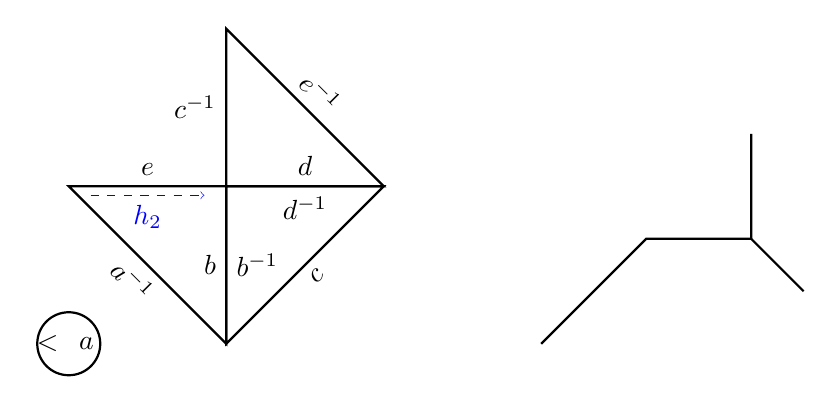
\begin{tikzpicture}[line width=0.8pt]
\foreach \i in {-9,...,9}{
	\foreach \j in {-9,...,9}{
		\coordinate(v\i\j) at (\i,\j);
		\foreach \k in {1,...,8}{
			\coordinate(v\i\j\k) at ($(v\i\j)+(\k*45-22.5: 0.3)$);
		}
	}
}

\draw (v-42)--(v-20)node[midway,sloped, below]{$a^{-1}$}--(v-22)node[midway, left]{$b$}--cycle node[midway, sloped, above]{$e$};
\draw (v-20)--(v-22)node[midway, right]{$b^{-1}$}--(v02)node[midway, sloped, below]{$d^{-1}$}--cycle node[midway, sloped, below]{$c$};
\draw (v-22)--(v02)node[midway,above]{$d$}--(v-24)node[midway, sloped, above]{$e^{-1}$}--cycle node[midway,left]{$c^{-1}$};
\draw (v-40) circle (0.4) node[left]{$<$} node[right]{$a$};
\draw [line width=0.2pt, blue, dashed,->] (v-428)--(v-225)node[midway,below]{$h_2$};

%\draw (v20)--(v31)--(v51)--(v53);
\draw (2,0)--(4/3+2,4/3)--(8/3+2,4/3)--(8/3+2,8/3);
\draw (8/3+2,4/3)--(10/3+2,2/3);
\end{tikzpicture}
\caption{Reduction of the words $a$, $a^{-1}eb$, $b^{-1}d^{-1}c$ and $c^{-1}de^{-1}$.}
\end{figure}
\end{document}



